\section{Bewertung des MOT-Systems} \label{sec:Meth MOT}
Mit eine \gls{MOT} System sollen \gls{Trajektorie}[n] generiert werden um diese für \gls{Feature}[s] zu nutzen. In \ref{sec:Meth DefAufgabe} wird dargestellt, dass die Merkmale der Verhaltensweisen stark auf der Bewegung der Puten basieren. Über die \gls{Trajektorie}[n] sollen diese Informationen extrahiert werden können. Um das zu gewährleisten muss das \gls{MOT} System gut genug sein, um die Bewegungsmerkmale jeglicher Verhaltensweisen zu erfassen. Dies ist durch die Bewertung des \gls{MOT} Systems zu überprüfen. \par

Für die Evaluation des \gls{MOT} Systems ist eine \gls{Ground Truth} notwendig. Da die Evaluation Gültigkeit für einen sehr konkreten Anwendungsfall haben soll, ist es sinnvoll eine anwendungsbezogene \gls{Ground Truth} zu verwenden, anstatt Benchmarking Datensätze. \gls{Ground Truth}[s] für zwei Ereignisse wurden bereits vor dieser Arbeit erstellt. Wie in \ref{sec:MOT GT} dargestellt ist die Erstellung einer qualitativ hochwertigen \gls{Ground Truth} herausfordernd. Um die Aussagekraft der Evaluation beurteilen zu können, wird die Qualität der \gls{Ground Truth} diskutiert. \par

Für das \glsdisp{Assoziation}{Assoziationsmodul} ist ein Algorithmus auszuwählen. Zur Auswahl steht der \acrshort{SORT} Algorithmus (\autoref{sec:MOT SORT}) und eine modifizierte Variante des Crocker-Grier Linking Algorithmus (\autoref{sec:MOT CrockGrier}). Die Modifikationen werden in \autoref{sec:Meth CrockGrieMods} erläutert. Für das Gesamtsystem ist zu Bewerten, welcher der Algorithmen die besten \gls{Feature}[s] gewährleisten kann. \par

Während der Versuche werden die Laufzeiten der Algorithmen gemessen, da diese relevant sind im Bezug auf die Echtzeitfähigkeit des Moduls. 


\subsection{Diskussion der Ground Truth Qualität} \label{sec:Meth GT Quali}
Noch vor dieser Arbeit sind zu zwei Ereignissen \gls{Ground Truth}[s] erstellt worden. Ein Kampfereignis und ein Kontrollgangereignis. Die Ereignisse sind jeweils eine Minute lang. Das Kampfereignis umfasst 91 \gls{Frame}[s], das Kontrollgangereignis umfasst 98 \gls{Frame}[s]. Dadurch ergiebt sich eine durchschnittliche \gls{Frame}[rate] von 1,6 \gls{Frame}[s] pro Sekunde. Die Ereignisse wurden von unterschiedlichen Personen bearbeitet.  \par

Die Herausforderungen, die die Erstellung einer qualitativ hochwertigen \gls{Ground Truth} mit sich bringt, waren zum Zeitpunkt der Erstellung nicht bewusst. Aus diesem Grund wurden keine klar definierten Regeln festgelegt, wie mit Mehrdeutigkeiten und anderen komplizieren Situationen umzugehen ist. Ganz ohne Regeln erfolgte die Erstellung jedoch nicht. Im Vorfeld wurde definiert, dass jedes Tier mit einer rechteckigen \gls{Bounding Box} zu \glsdisp{Detektion}{detektieren} ist. Die \gls{Bounding Box} soll das Tier möglichst eng, aber vollständig umschließen. Tiere sollen möglichst auch nach Verdeckungen korrekt \glsdisp{Assoziation}{assoziiert} werden. \par 

Bei der Überprüfung der \gls{Ground Truth} viel auf, die \gls{Detektion} funktionierte relativ zuversichtlich. Auch die \gls{Lokalisation} ist zufriedenstellend, auch wenn Schwankungen zu erwarten sind. Schwächen sind vor allem bei Mehrdeutigkeiten vorhanden. Die \gls{Detektion} bei teilweisen Verdeckungen ist inkonstant. Auch haben die unterschiedlichen Bearbeiter mehrdeutige Situationen unterschiedlich gelöst. Dadurch ist zu erwarten, dass Unsicherheiten in der Bewertung des \gls{Detektion}[smoduls] entstehen. Die Überprüfung zeigte, dass die \gls{Ground Truth} tendenziell eher Übermäßig optimistische Erwartungen an die \gls{Detektion} stellt. Bei teilweisen Verdeckungen wurde ein Tier länger \glsdisp{Detektion}{detektiert}, als es das \gls{Detektion}[smodul] tat. Somit ist mit einer vermehrten Anzahl von falsch negativen \gls{Detektion}[en] (\autoref{sec:MOT Fehlertypen}) zu rechnen. \par

Die niedrige \gls{Frame}[rate], sowie die hohe Tierdichte im Stall, sorgten dafür das sich Tiere teilweise nur schwer auseinander halten ließen. Dadurch ist mit Unsicherheiten in der Evaluation des \gls{Assoziation}[smoduls] zu rechnen. 

Es ist empfehlenswert, dass das \gls{Detektion}[smodul] mit Daten trainiert wird, die aus der gleichen Quelle stammen wie die \gls{Ground Truth}. Das stellt eine faire Bewertung sicher, da keine diskrepanz vorhanden ist zwischen dem was das \gls{Detektion}[smodul] lernt und dem was die Evaluation von ihm fordert. Dies war hier nicht möglich, da die \gls{Detektion} bereits abgeschlossen war als die \gls{Ground Truth} erstellt wurde. Dadurch ist mit Unsicherheiten der Bewertung des \gls{Detektion}[smoduls] und des \gls{Lokalisation}[smoduls] zu rechnen.\par

Mit Fehlern in einer \gls{Ground Truth} ist zu rechnen. Um dennoch stabile Ergebnisse zu erhalten wird empfohlen mehrere \gls{Ground Truth}[s] zu verwenden und die Ergebnisse zu mitteln. Für die Bewertung bezogen auf den Anwendungsfall stehen jedoch nur zwei \gls{Ground Truth} Datensätze zur Verfügung. Das kann die Stabilität der Wertungen negativ beeinflussen.


\subsection{Modifikation des Crocker-Grier Linking Algorithmus} \label{sec:Meth CrockGrieMods}
Der grundlegende Aufbau des Crocker-Grier Linking Algorithmus ist in \autoref{sec:MOT CrockGrier} erläutert. Die Modifikationen erfolgten bereits vor dieser Arbeit. Sie werden hier erläutert, um die Nachvollziehbarkeit der Arbeitsweise zu ermöglichen. \par

Bei der Anwendung der ursprünglichen Form des Crocker-Grier Linking Algorithmus auf Ereignisse im Putenmaststall, kam es zu Problemen. Die maximale Distanz \(l\) die ein Objekt zwischen zwei \gls{Frame}[s] zurücklegen darf, um korrekt \glsdisp{Assoziation}{assoziiert} werden zu können, wird von den Tieren oftmals nicht eingehalten. Gerade bei dynamischen Ereignissen legen die Puten in kürzerer Zeit, weitere Strecken zurück. Dies ist auch der niedrigen \gls{Frame}[rate] und hohen Tierdichte geschuldet. Durch die Verletzung von \(l\) entstehen \gls{Assoziation}[sfehler] (\autoref{sec:MOT Fehlertypen}). Durch die Vergrößerung von \(l\) entstehen größere Netzwerke. In der Anwendung wurden die Netzwerke schnell so groß, dass die Rechenzeit unpraktikabel wurde.\par

Um diesen Problemen zu begegnen wurde eine iterative \gls{Assoziation} umgesetzt. Diese durchläuft mehrere Stufen, in denen die \gls{Assoziation} wiederholt wird. Bei jeder Iteration wird \(l\) vergrößert. Korrekte \gls{Assoziation}[en] werden in den folgenden Stufen nicht mehr betrachtet. Insgesamt werden drei Iterationen durchlaufen. Die Abbildung \ref{fig:funkCrockGrierMod} zeigt die Auswirkungen dieses Ansatzes. In der ersten Stufe werden vor allen stationäre Puten \glsdisp{Assoziation}{assoziiert}. Diese werden in den folgenden Stufen nicht mehr betrachtet. Dadurch wird der Abstand zwischen den zu \glsdisp{Assoziation}{assoziierenden} Objekten größer und korrekte \gls{Assoziation}[en] sind auch mit einem größeren \(l\) zu erwarten. Auch die Größen der entstehenden Netzwerke sind besser handhabbar. 

\begin{figure}[htb]
    \centering
    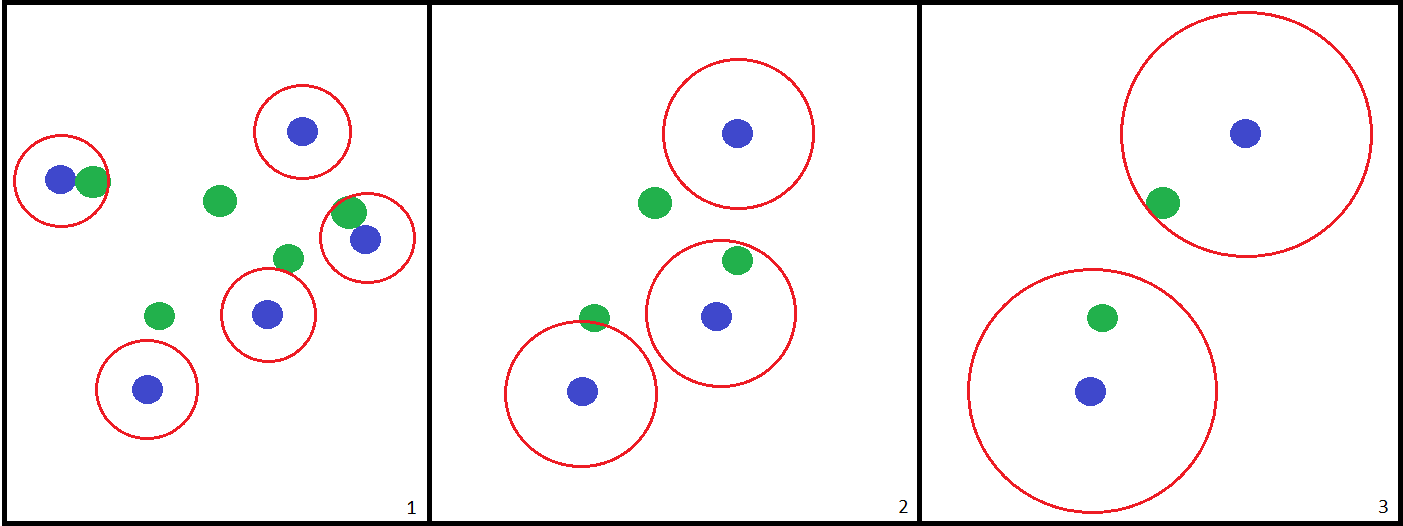
\includegraphics[width=0.9\textwidth]{img/Grafiken/CrockGrierMod Funktionsprinzip.png}
    \caption[Ansatz der Modifikationen des Crocker-Grier Linking Algorithmus.]{Ansatz der Modifikationen des Crocker-Grier Linking Algorithmus.}
    \label{fig:funkCrockGrierMod}
\end{figure}

Gerade bei hoch dynamischen Ereignissen passiert es, dass in frühen Stufen nur wenige \gls{Assoziation}[en] getätigt werden können. Dadurch entstehen wieder mehr \gls{Assoziation}[sfehler]. Auch ist nicht mehr zu gewährleisten, dass der Rechenaufwand handhabbar bleibt. Aus diesem Grund wird in diesen Situationen das adaptive Verfahren angewendet, was in der \gls{Bibliothek} \textit{Trackpy} \cite{Allan.2023} implementiert ist. Dadurch wird sichergestellt, dass die Netzwerke eine Maximalgröße nicht überschreiten und der Rechenaufwand bleibt handhabbar. \par

Ziel ist es konstante \gls{Trajektorie}[n] zu generieren. Durch die Iterationen der Stufen können jedoch \gls{Fragmentation}[sfehler] provoziert werden. Das ist in der Abbildung \ref{fig:bspCrockGrierFrag} dargestellt. Unterbricht ein aktives Tier seine dynamische Bewegung für Wenige \gls{Frame}[s] und verweilt auf einer Position, dann werden die \gls{Assoziation}[en] dieser wenigen \gls{Frame}[s] bereits in einer früheren Stufe getätigt. Die \gls{Detektion}[en] der dynamischen Bewegung werden erst in höheren Stufen \glsdisp{Assoziation}{assoziiert}. Eine konstante \gls{Trajektorie} ist dann nicht mehr möglich, da das Verweilen des Tieres bereits aus der weiteren Betrachtung herausgenommen wurde. 

\begin{figure}[htb]
    \centering
    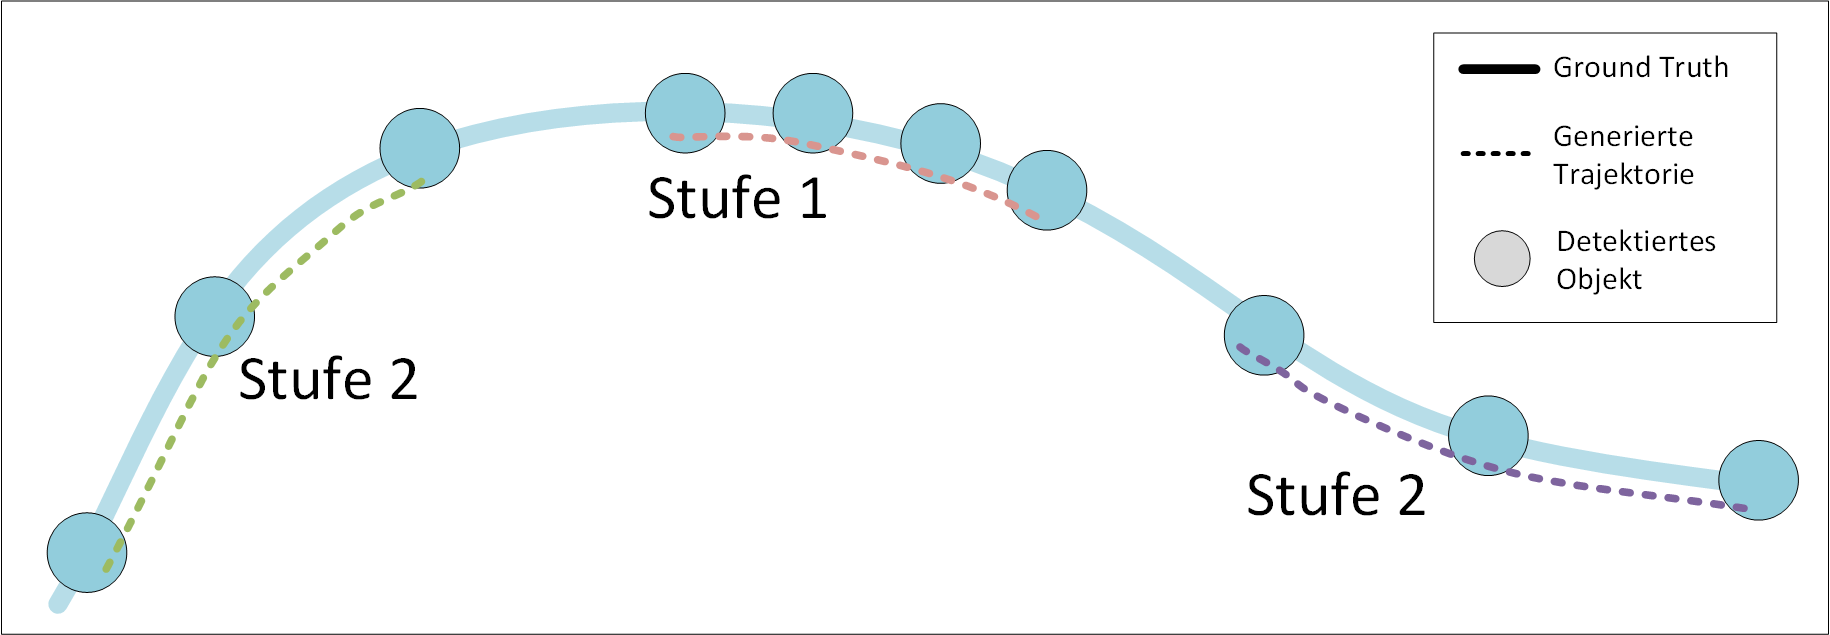
\includegraphics[width=0.9\textwidth]{img/Grafiken/Fragmentation durch Stufen.png}
    \caption[Fragmentation durch die Modifikationen des Crocker-Grier Linking Algorithmus.]{Fragmentation durch die Modifikationen des Crocker-Grier Linking Algorithmus. Durch Veränderungen in der Geschwindigkeit werden zusammengehörende Detektionen in anderen Stufen assoziiert.}
    \label{fig:bspCrockGrierFrag}
\end{figure}

Um solche Fehler zu vermeiden wurde ein Verifikatoinsmechanismus eingeführt, welcher evaluiert, ob eine \gls{Trajektorie} in einer bestimmten Stufe plausibel ist, oder nicht. ist die \gls{Trajektorie} plausibel, gilt sie als verifiziert und sie wird in das Ergebnis des \gls{MOT} Systems aufgenommen. Kann die \gls{Trajektorie} nicht verifiziert werden, dann kommen ihrer \gls{Detektion}[en] in die nächste Stufe. \gls{Detektion}[en], welche sich am Ende nicht in einer verifizierten \gls{Trajektorie} befinden, werden verworfen. Die Abbildung \ref{fig:TreeCrockGrierVerif} zeigt den Verifkationsmechanismus in Form eines Baumdiagramms. 

\begin{figure}[H]
    \centering
    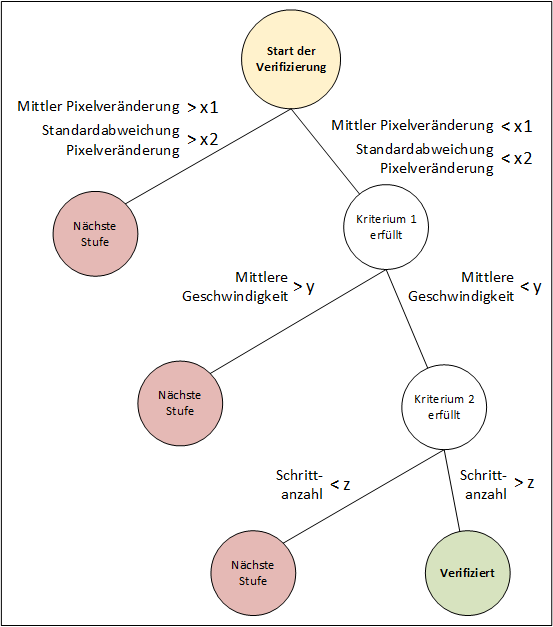
\includegraphics[width=0.8\textwidth]{img/Grafiken/Baumdiagramm Verifizierung der Trajektorien.png}
    \caption[Baumdiagramm der Verifikation des modifizierten Crocker-Grier Algorithmus.]{Baumdiagramm des Verifikationsmechanismus des modifizierten Crocker-Grier Linking Algorithmus.}
    \label{fig:TreeCrockGrierVerif}
\end{figure}

Für die Verifikation wird das Video des Ereignisses mit herangezogen. Bei diesem wird ermittelt wie sich die Pixeln von \gls{Frame} zu \gls{Frame} verändern. Wenn \(\nommat{PIX}_t\) die Matrix aller Pixel in einem \gls{Frame} \(t\) ist, dann berechnet sich die Veränderung wie in \autoref{eq:Pixelveränderung} dargestellt.

\begin{equation}
\text{Pixelveränderung} = \frac{\sum_i \sum_j |pix_{t_{i,j}} - pix_{{t-1}_{i,j}}|}{\text{Pixelanzahl}}
\label{eq:Pixelveränderung}
\end{equation}

Dabei werden die Farbkanäle berücksichtigt. Ein \(Pixel \in \nommat{PIX}\) besitzt jeweils einen Kanal für rot, blau und grün. Diese können die Werte \(\{0,1,2, \dots, 255\}\) annehmen. Mathematisch lässt sich jeder Pixel als Vektor \(\nomvec{pix}\) betrachten. Der Wertebereich der Pixelveränderung somit \([0, 765]\), da \(3 \cdot 255 = 765\). \par

Der Verlauf der Pixelveränderung wird für das Ereignis ermittelt. Sie dient als Aktivitätsindikator. Eine \gls{Trajektorie} muss nicht über das gesamte Ereignis verlaufen. Es wird der Zeitraum betrachtet, in dem die \gls{Trajektorie} aktiv war. Für diesen Zeitraum wird die mittlere Pixelveränderung berechnet und die Standdardabweichung. Diese Werte dienen dazu um zu beurteilen, ob das Geschehen im Stall insgesamt Dynamisch ist, oder nicht. Bei einem dynamischen Geschehen, wie bei einem Kontrollgang, ist es sinnvoll die \gls{Detektion}[en] bei einem größeren \(l\) zu betrachten, da \gls{Fragmentation}[sfehler] wahrscheinlicher sind. \par

Die mittlere Geschwindigkeit aller \gls{Trajektorie}[n] wird berechnet und die Geschwindigkeit der individuellen \gls{Trajektorie}[n] wird damit verglichen. Liegt die Geschwindigkeit auffällig höher, als die mittlere Geschwindigkeit, wird das Potential für \gls{Fragmentation}[sfehler] als höher eingestuft und die \gls{Detektion}[en] werden in der nächsten Stufe erneut beurteilt. \par

Das letzte Verifikationskriterium ist die Schrittanzahl der \gls{Trajektorie}[n]. Von \gls{Trajektorie}[n], die über viele \gls{Frame}[s] verlaufen ist tendenziell zu erwarten, dass sie konstanter sind. Somit fordert der Verifikationsmechanismus eine minimale \gls{Frame}[anzahl], oder Anzahl von Zeitschritten.\par

Die Die Verifikationskriterien der unterschiedlichen Stufen sind dynamisch. Da in höheren Stufen eine höhere Fehleranfälligkeit erwartet wird, sinkt die minimale \gls{Frame}[anzahl], um nicht zu viele \gls{Trajektorie}[n] auszusortieren. Auch die Toleranzschranken für die Dynamik steigen, da in den höheren Stufen mehr Dynamik erwartet wird. \par



\subsection{Methodisches Vorgehen der MOT Evaluationen}
Für die Evaluation stehen zwei \gls{Ground Truth} Ereignisse zur Verfügung. Ein Kampfereignis und ein Kontrollgangereignis (\autoref{sec:Meth GT Quali}). Die Algorithmen, zwischen denen Auszuwählen ist sind der \acrshort{SORT} Algorithmus (\autoref{sec:MOT SORT}) und die modifizierte Variante des Crocker-Grier Linking Algorithmus (\autoref{sec:Meth CrockGrieMods}). Die Evaluation wird mittels der \gls{HOTA} Metrik (\autoref{sec:MOT HOTA}) durchgeführt, da mit dieser Metrik die fairste Bewertung zu erwarten ist und die genausten Fehleranalysen. Die \textit{\gls{IDF1}-Metrik} und die \textit{\acrshort{CLEAR} \gls{MOT}} Metriken werden jedoch angegeben, da sie etablierter sind als \gls{HOTA}. Für die Berechnung der Metriken wird die Software \textit{TrackEval} benutzt \cite{TrackEval.2020}. Diese ist die offizielle Evaluationsoftware der \textit{MOTChallenge} und steht als Open-Source Code zur Verfügung. Mit der Nutzung von \textit{TrackEval} wird sichergestellt, dass die Metriken korrekt berechnet werden. \par

Als erstes wird für beide Algorithmen die Gesamtperformance bewertet. Dazu werden die beiden Algorithmen auf die Ereignisse angewendet zu denen \gls{Ground Truth}[s] vorhanden sind. Für jeden \gls{Assoziation}[salgorithmus] ist anschließend ein Trackingergebnis vorhanden. Dieses beinhaltet die \gls{Trajektorie}[n]. Gespeichert werden die Trackingergebnisse als txt-Datei. Die Formatierung erfolgt angepasst an \textit{TrackEval}, gemäß \cite{MOT15}. Anschließend werden die Metriken berechnet. Wie \textit{TrackEval} auf eigene \gls{MOT} Systeme und mit eigenen \gls{Ground Truth}[s] anzuwenden ist, ist in der Dokumentation erläutert \cite{TrackEval.2020}. Die Evaluation der beiden Ereignisse wird gemittelt. Die Ergebnisse der beiden Algorithmen lassen sich vergleichen. Neben den Wertungen der \gls{HOTA} Metrik, erstellt \textit{TrackEval} einen Plot. Dieser zeigt den Verlauf der Wertungen über \(\alpha\). Die Abbildung \ref{fig:MPNTrack} zeigt einen solchen Plot. Dieser ist einem \gls{MOT} System namens \textit{MPNTrack} entnommen, welcher bei der \textit{MOTChallenge} 2016 und 2017 angetreten ist. Dieser ist hier zu Beispielzwecken angeführt. 

\begin{figure}[htb]
    \centering
    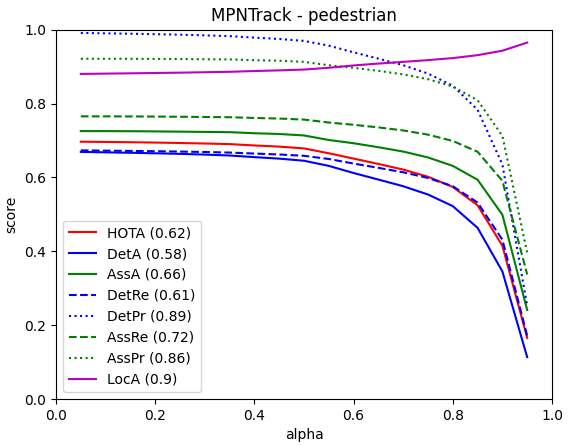
\includegraphics[width=0.9\textwidth, height=11cm]{img/Plots/MPNTrack MOT17.png}
    \caption[Beispiel eines Evaluationsergebnisses eines MOT Systems mit der HOTA Metrik.]{Beispiel eines Evaluationsergebnisses eines MOT Systems mit der HOTA Metrik.}
    \label{fig:MPNTrack}
\end{figure}

Während der Generation der Trajektorien werden die Laufzeiten der Algorithmen gemessen. Ebenfalls werden weitere Laufzeitmessungen durchgeführt, bei denen die Länge der Ereignisse stärker zu variieren sind. Dadurch ist ein Vergleich der Laufzeiten möglich und auch wie die Laufzeiten im Bezug auf die Ereignisslänge Skalieren.\par 

Als nächstes ist zu überprüfen, ob die \gls{Assoziation}[salgorithmen] alle Verhaltensweisen 
gleich gut \glsdisp{Assoziation}{assoziiert} bekommen. Dazu wird jedes Ereignis unabhängig von einander evaluiert.\par
